\documentclass{standalone}
\usepackage{tikz}
\usetikzlibrary{calc, shapes, patterns}

\begin{document}
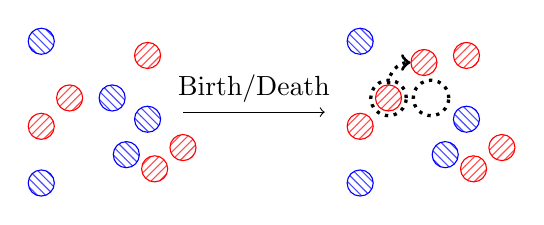
\begin{tikzpicture}[scale=.9]
	\node (A1) at (-1, -1) [circle, pattern=north west lines, pattern
        color=blue!70, draw=blue] {};
	\node (A2) at (-1, 1) [circle, pattern=north west lines, pattern
        color=blue!70, draw=blue] {};
	\node (A3) at (0, .2) [circle, pattern=north west lines, pattern
        color=blue!70, draw=blue] {};
	\node (A4) at (.2, -.6) [circle, pattern=north west lines, pattern
        color=blue!70, draw=blue] {};
	\node (A5) at (.5, -0.1) [circle, pattern=north west lines, pattern
        color=blue!70, draw=blue] {};
	\node (B1) at (-1, -.2) [circle, pattern=north east lines, pattern
        color=red!70, draw=red] {};
	\node (B2) at (1, -.5) [circle, pattern=north east lines, pattern
        color=red!70, draw=red] {};
	\node (B3) at (.5, .8) [circle, pattern=north east lines, pattern
        color=red!70, draw=red] {};
	\node (B4) at (-.6, .2) [circle, pattern=north east lines, pattern
        color=red!70, draw=red] {};
	\node (B5) at (.6, -.8) [circle, pattern=north east lines, pattern
        color=red!70, draw=red] {};

	\draw [->] (1, 0) -- (3, 0) node [above, pos=0.5] {Birth/Death};

	\node (A1) at ($(A1) + (4.5, 0)$) [circle, pattern=north west lines,
        pattern color=blue!70, draw=blue] {};
	\node (A2) at ($(A2) + (4.5, 0)$) [circle, pattern=north west lines,
        pattern color=blue!70, draw=blue] {};
	\node (A3) at ($(A3) + (4.5, 0)$) {};
	\node (A4) at ($(A4) + (4.5, 0)$) [circle, pattern=north west lines,
        pattern color=blue!70, draw=blue] {};
    \node (A5) at ($(A5) + (4.5, 0)$) [circle, pattern=north west lines,
        pattern color=blue!70, draw=blue] {};
	\node (B1) at ($(B1) + (4.5, 0)$) [circle, pattern=north east lines,
        pattern color=red!70, draw=red] {};
	\node (B2) at ($(B2) + (4.5, 0)$) [circle, pattern=north east lines,
        pattern color=red!70, draw=red] {};
	\node (B3) at ($(B3) + (4.5, 0)$) [circle, pattern=north east lines,
        pattern color=red!70, draw=red] {};
	\node (B4) at ($(B4) + (4.5, 0)$) [circle, pattern=north east lines,
        pattern color=red!70, draw=red] {};
	\node (B5) at ($(B5) + (4.5, 0)$) [circle, pattern=north east lines,
        pattern color=red!70, draw=red] {};

	\draw [dotted, very thick] (B4) circle (.25cm);
	\node (B6) at ($(B4) + (0.5, 0.5)$) [circle, pattern=north east lines,
        pattern color=red!70, draw=red] {};
	\draw [->, dotted, very thick] (B4) [out=90, in=180] to (B6);

	\draw [dotted, very thick] (A3) circle (.25cm);
\end{tikzpicture}
\end{document}
